\documentclass[12pt,letterpaper,boxed]{hmcpset}
\usepackage{float}
\restylefloat{figure}
\usepackage{graphicx}
\usepackage{amsmath}


\name{Lujia Zhang}
\class{CSSE 477}
\mailbox{CM 1405}
\assignment{Assignment 6}

\begin{document}

\section*{Task 3: Configure a resource}
\begin{figure}[H]
  \centering
  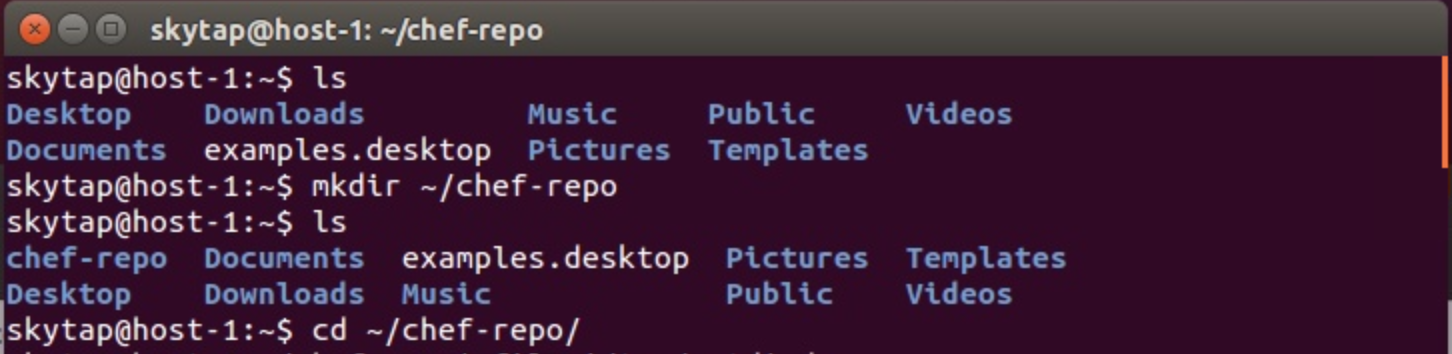
\includegraphics[width = 1.0\textwidth]{1.png}
\end{figure}
\begin{figure}[H]
  \centering
  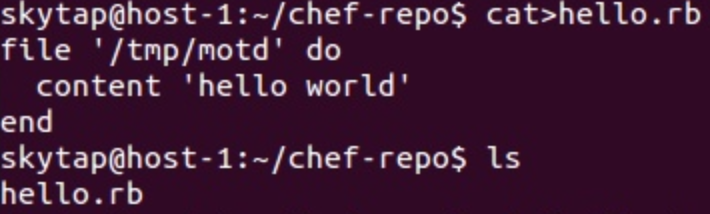
\includegraphics[width = 1.0\textwidth]{2.png}
\end{figure}
\begin{figure}[H]
  \centering
  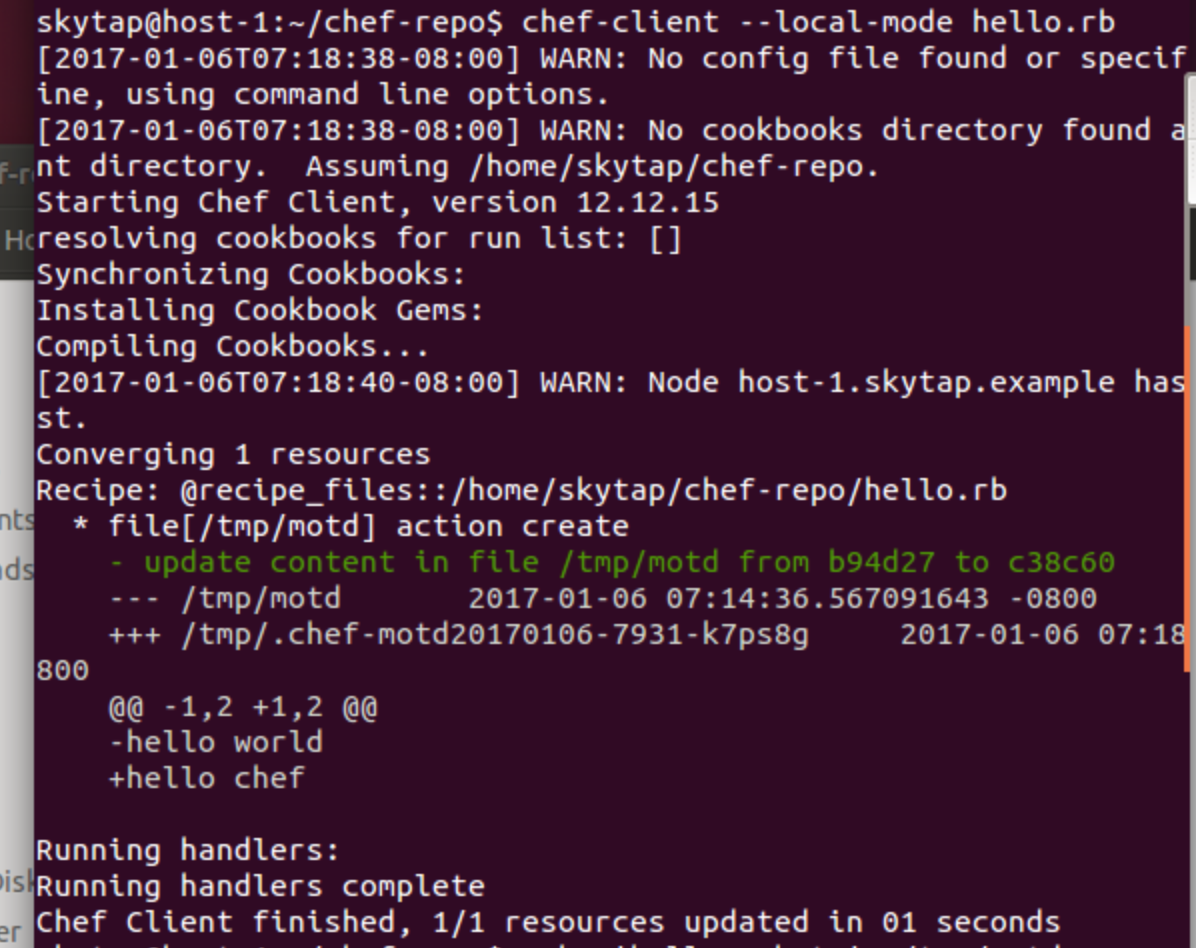
\includegraphics[width = 1.0\textwidth]{3.png}
\end{figure}
\begin{figure}[H]
  \centering
  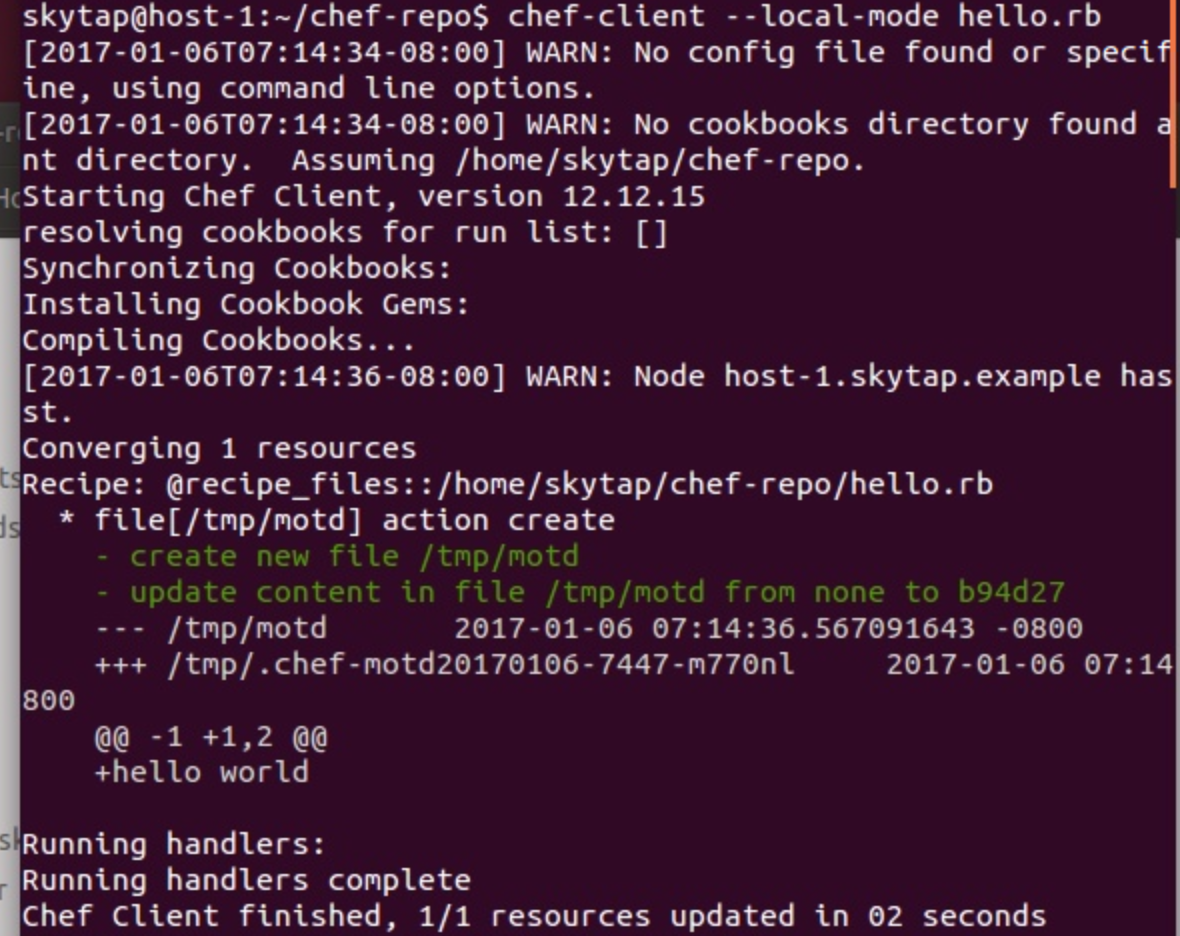
\includegraphics[width = 1.0\textwidth]{4.png}
\end{figure}
\begin{figure}[H]
  \centering
  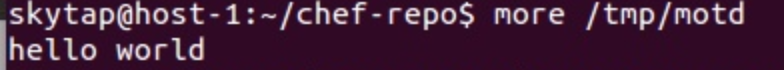
\includegraphics[width = 1.0\textwidth]{5.png}
\end{figure}
\begin{figure}[H]
  \centering
  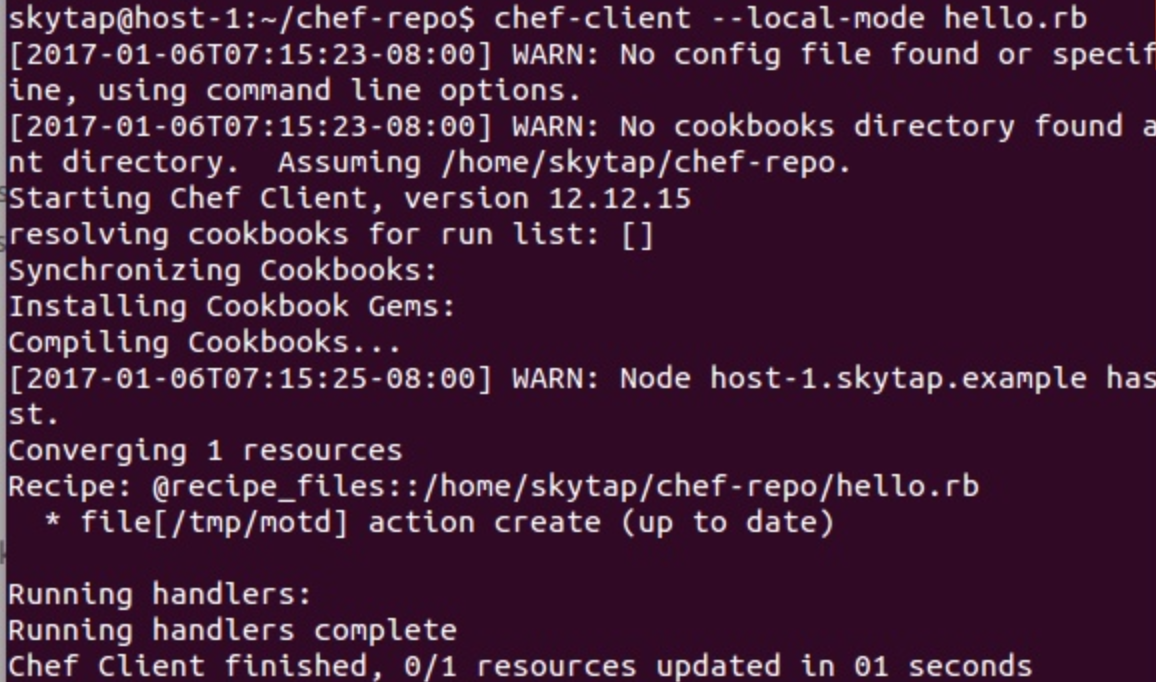
\includegraphics[width = 1.0\textwidth]{6.png}
\end{figure}
\begin{figure}[H]
  \centering
  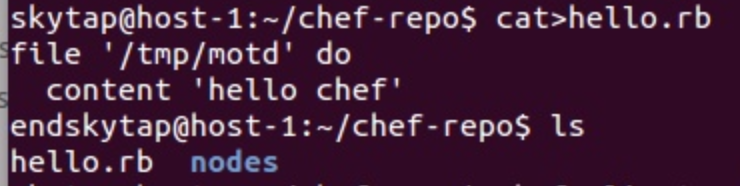
\includegraphics[width = 1.0\textwidth]{7.png}
\end{figure}
\begin{figure}[H]
  \centering
  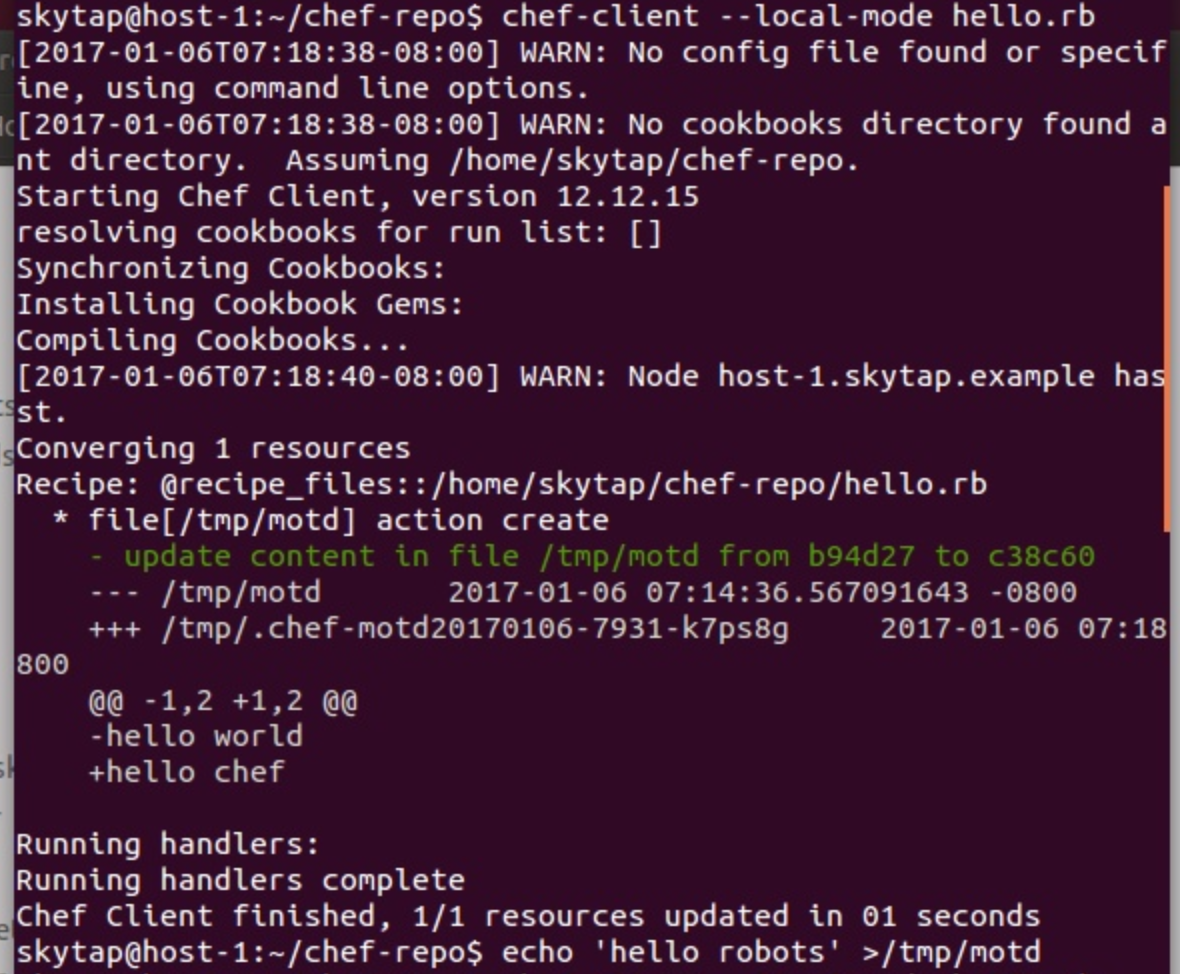
\includegraphics[width = 1.0\textwidth]{8.png}
\end{figure}
\begin{figure}[H]
  \centering
  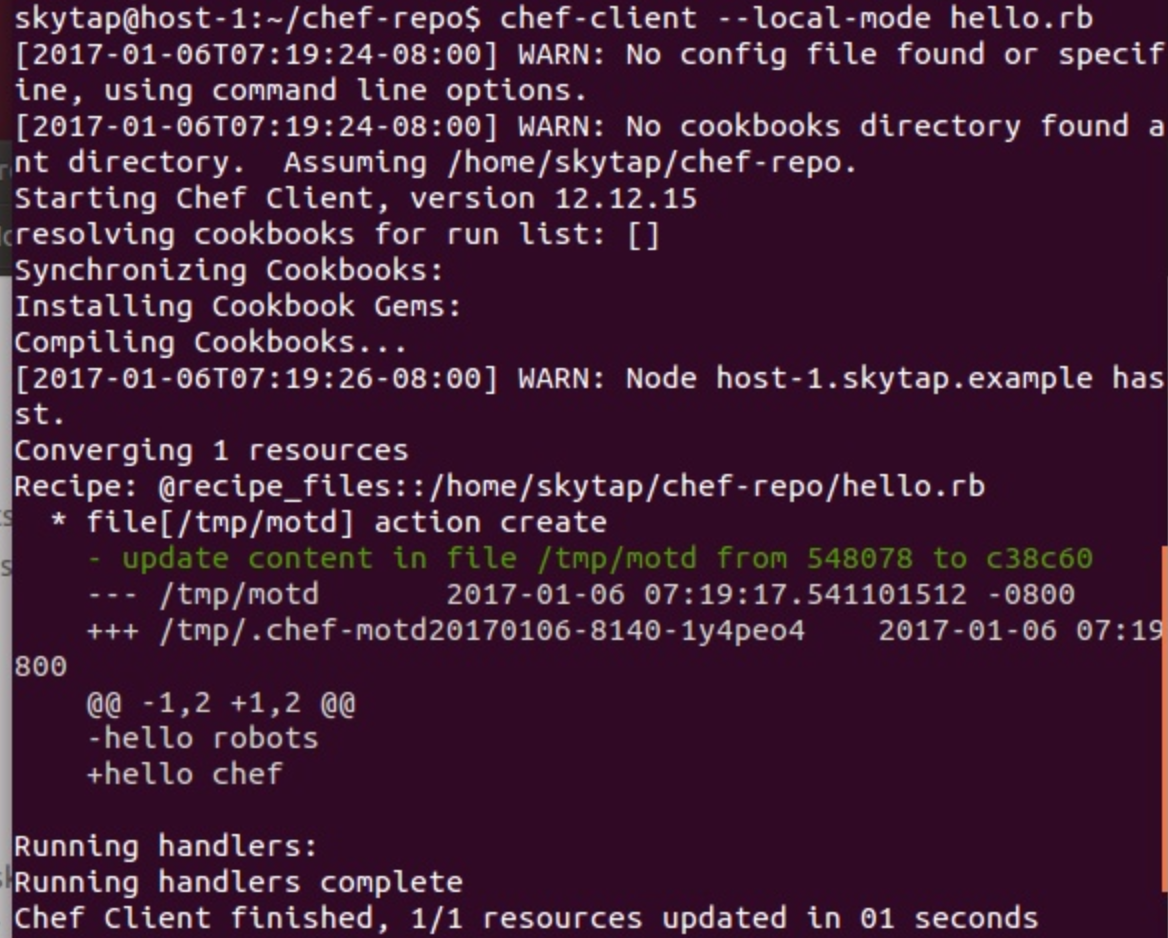
\includegraphics[width = 1.0\textwidth]{9.png}
\end{figure}
\begin{figure}[H]
  \centering
  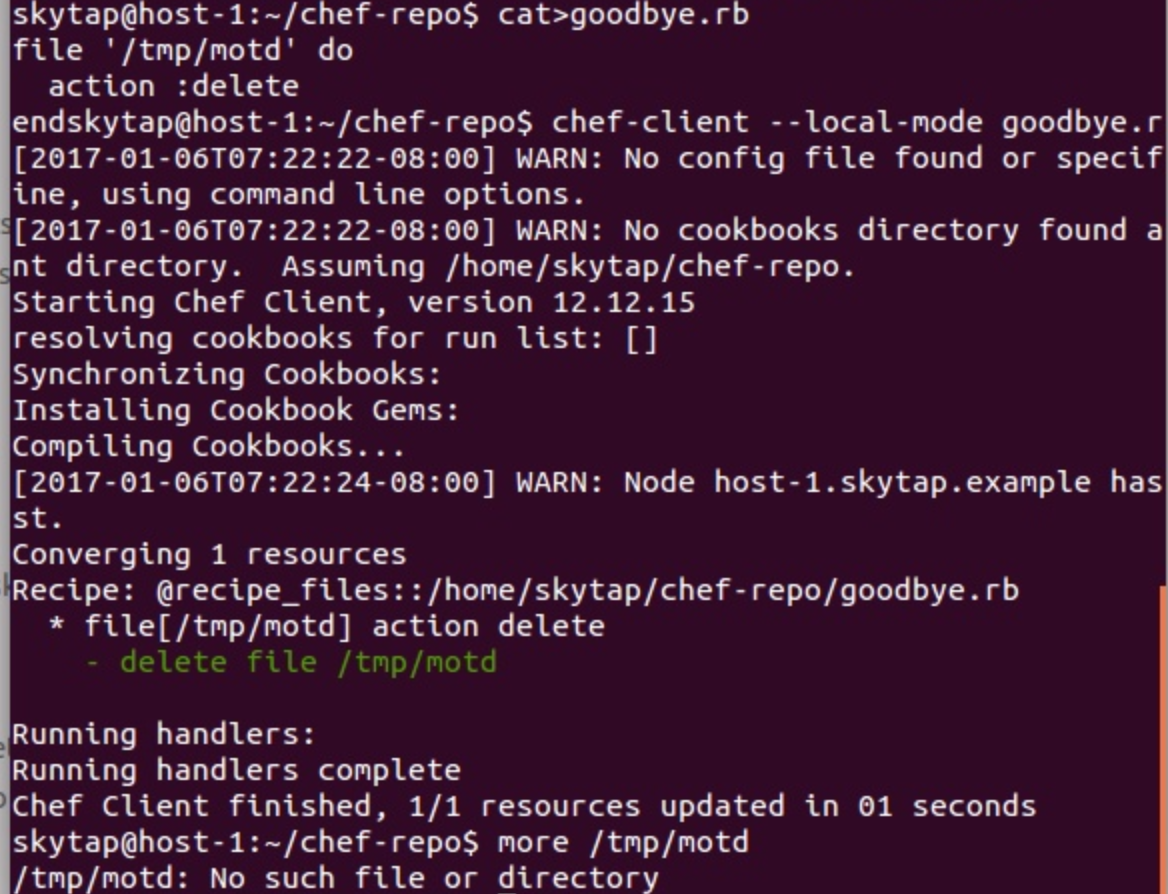
\includegraphics[width = 1.0\textwidth]{10.png}
\end{figure}
\begin{figure}[H]
  \centering
  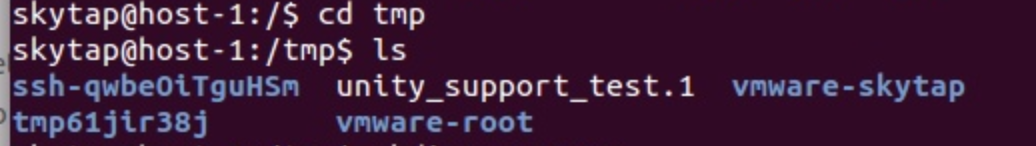
\includegraphics[width = 1.0\textwidth]{11.png}
\end{figure}
\begin{figure}[H]
  \centering
  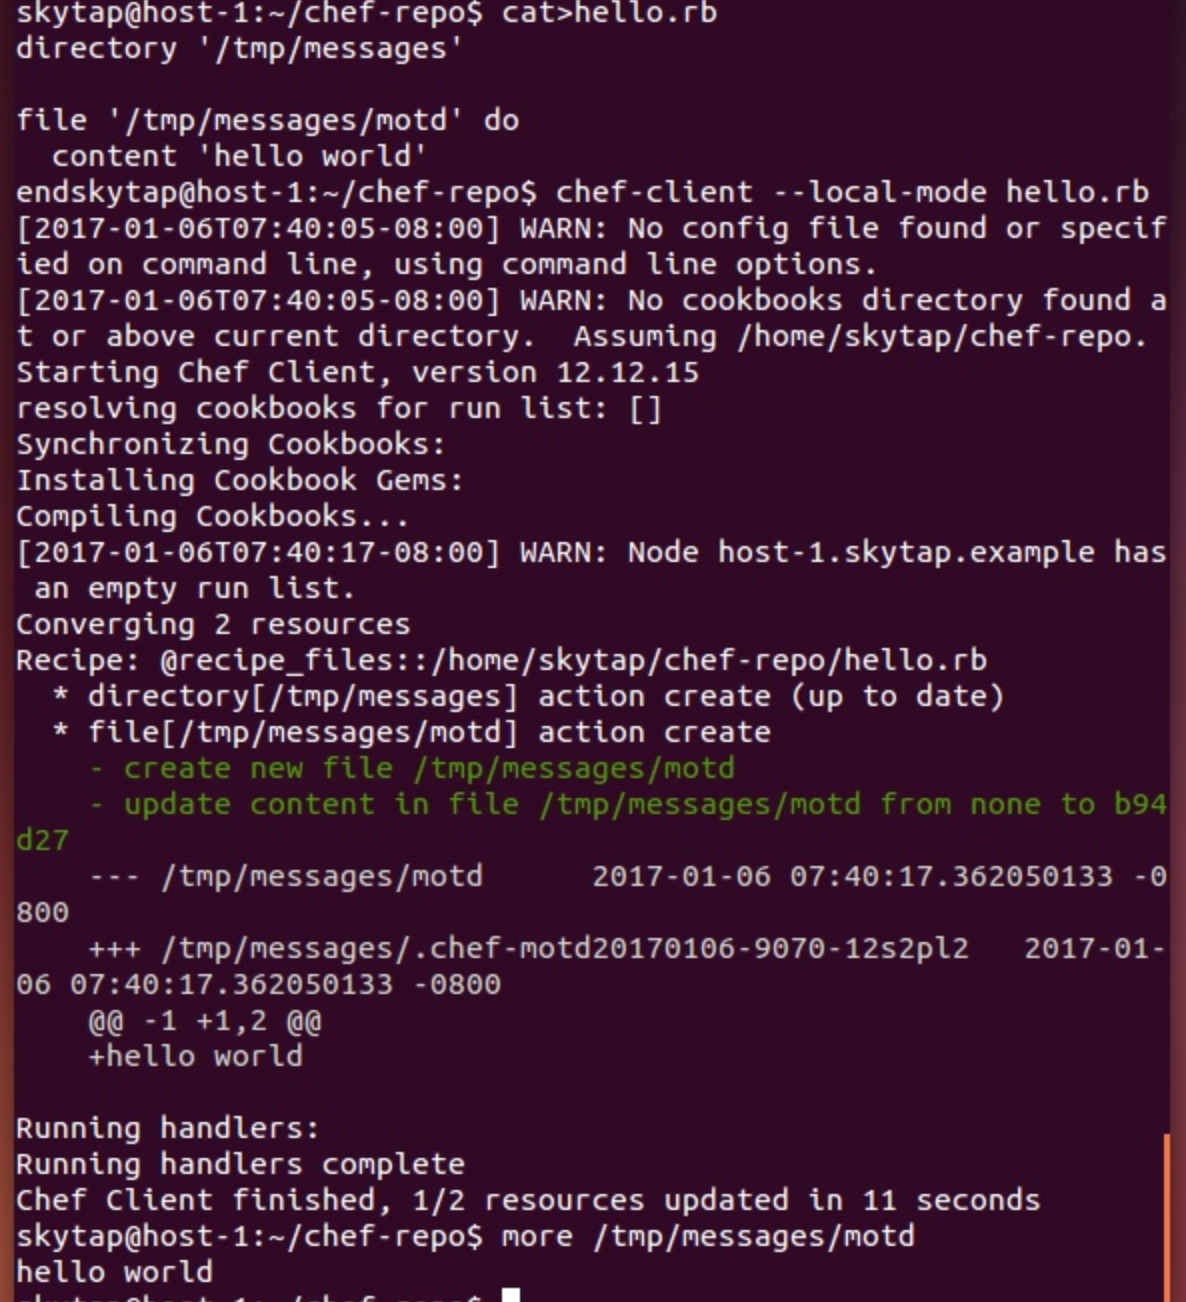
\includegraphics[width = 1.0\textwidth]{12.png}
\end{figure}

\section*{Task 4: Configure a package and service}
\begin{figure}[H]
  \centering
  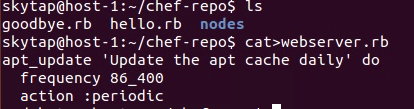
\includegraphics[width = 1.0\textwidth]{13.png}
\end{figure}
\begin{figure}[H]
  \centering
  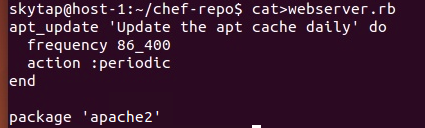
\includegraphics[width = 1.0\textwidth]{14.png}
\end{figure}
\begin{figure}[H]
  \centering
  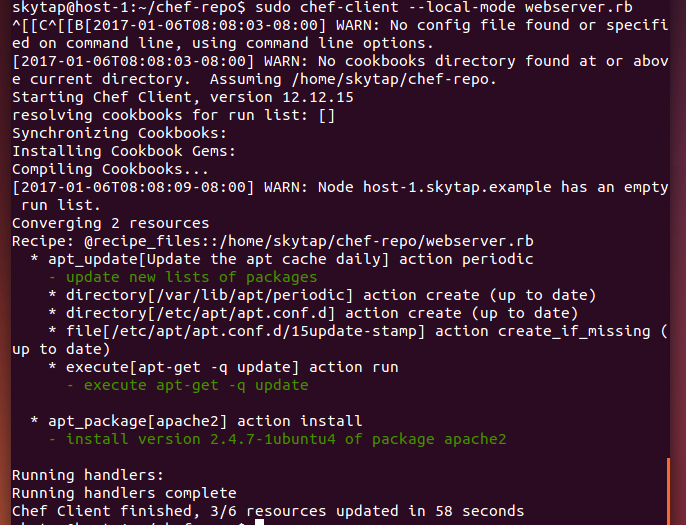
\includegraphics[width = 1.0\textwidth]{15.png}
\end{figure}
\begin{figure}[H]
  \centering
  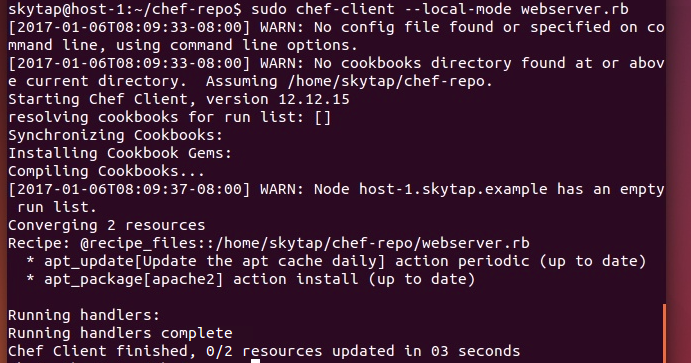
\includegraphics[width = 1.0\textwidth]{16.png}
\end{figure}
\begin{figure}[H]
  \centering
  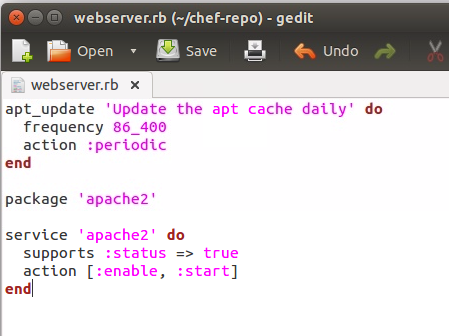
\includegraphics[width = 1.0\textwidth]{17.png}
\end{figure}
\begin{figure}[H]
  \centering
  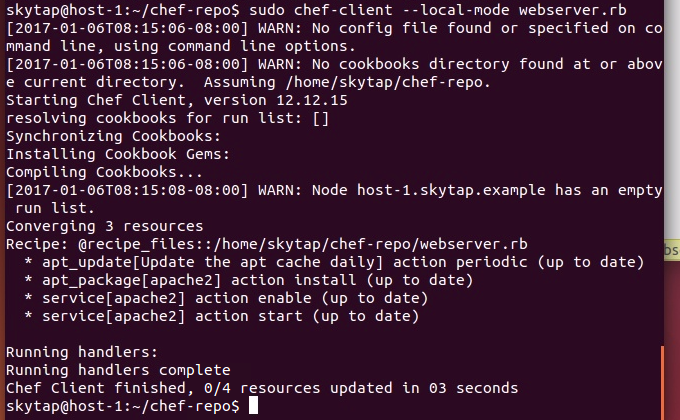
\includegraphics[width = 1.0\textwidth]{18.png}
\end{figure}
\begin{figure}[H]
  \centering
  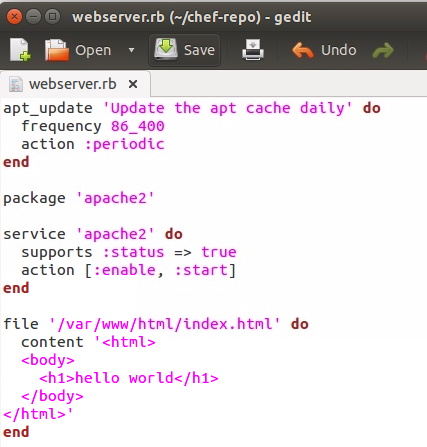
\includegraphics[width = 1.0\textwidth]{19.png}
\end{figure}
\begin{figure}[H]
  \centering
  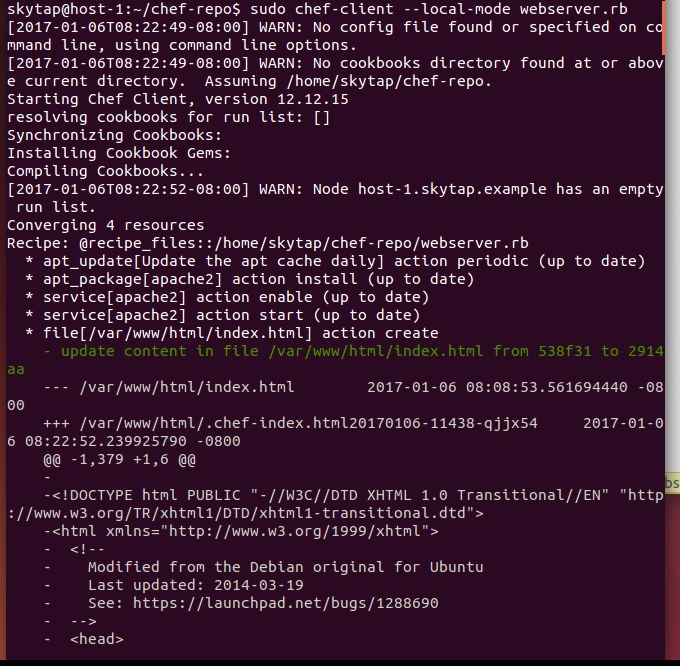
\includegraphics[width = 1.0\textwidth]{20.png}
\end{figure}
\begin{figure}[H]
  \centering
  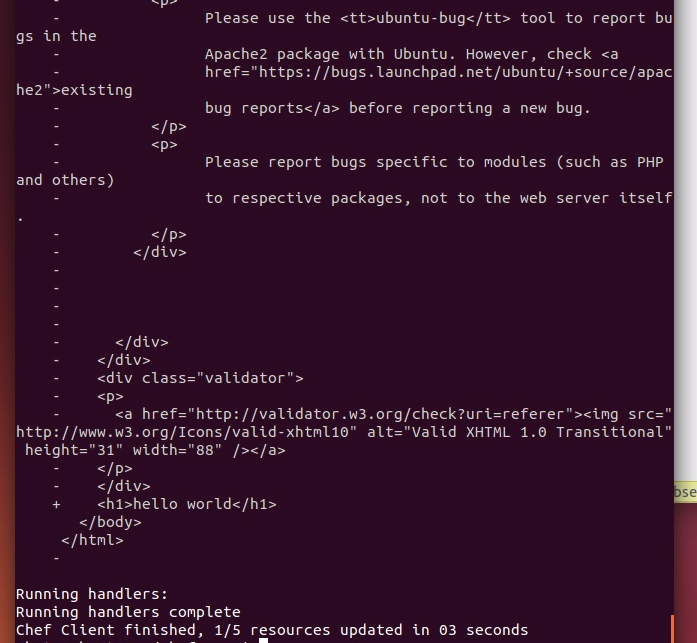
\includegraphics[width = 1.0\textwidth]{21.png}
\end{figure}
\begin{figure}[H]
  \centering
  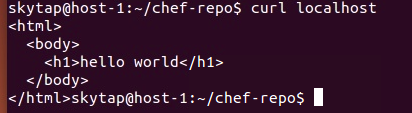
\includegraphics[width = 1.0\textwidth]{22.png}
\end{figure}
\begin{figure}[H]
  \centering
  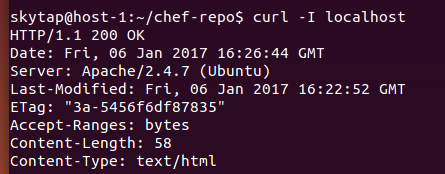
\includegraphics[width = 1.0\textwidth]{23.png}
\end{figure}
\begin{figure}[H]
  \centering
  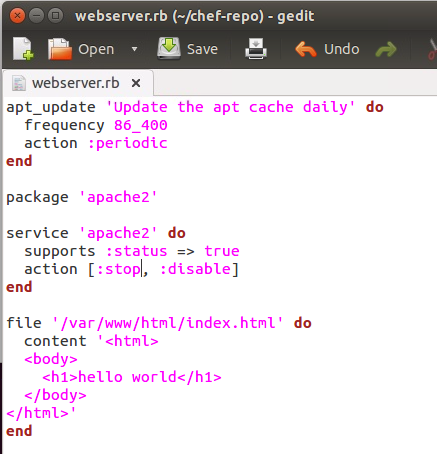
\includegraphics[width = 1.0\textwidth]{24.png}
\end{figure}
\begin{figure}[H]
  \centering
  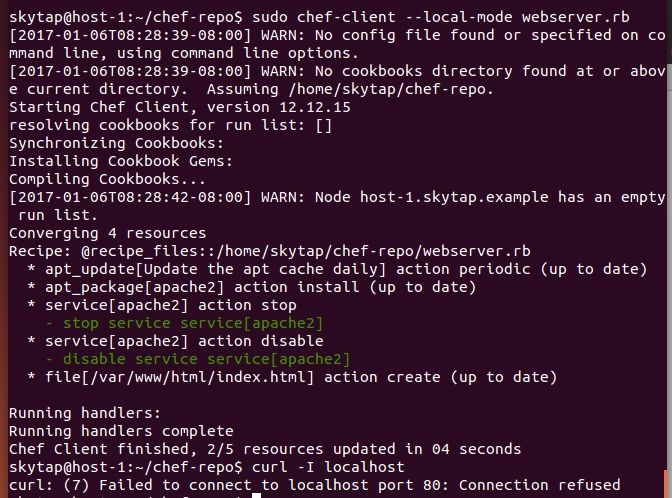
\includegraphics[width = 1.0\textwidth]{25.png}
\end{figure}

\section*{Task 5: Make your recipe more manageable }

\begin{figure}[H]
  \centering
  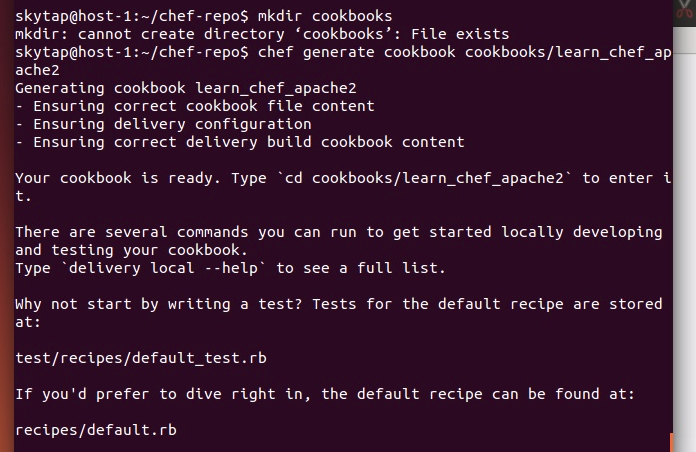
\includegraphics[width = 1.0\textwidth]{26.png}
\end{figure}
\begin{figure}[H]
  \centering
  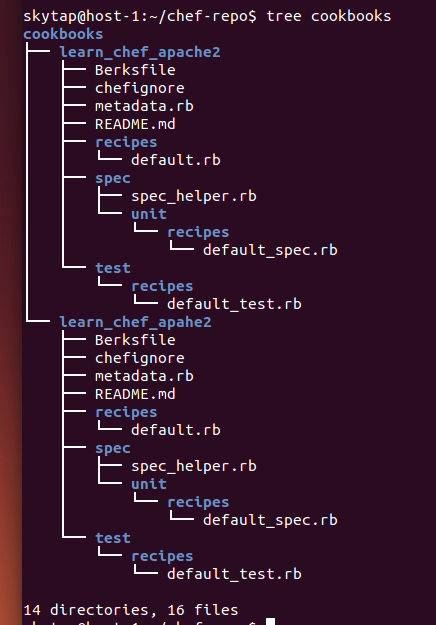
\includegraphics[width = 1.0\textwidth]{27.png}
\end{figure}
\begin{figure}[H]
  \centering
  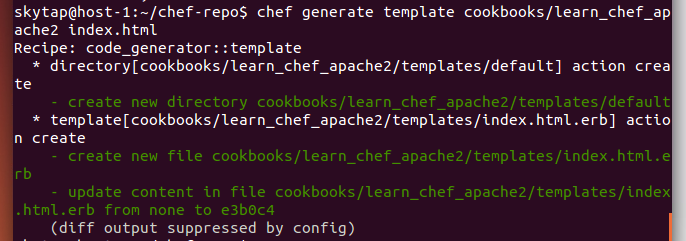
\includegraphics[width = 1.0\textwidth]{28.png}
\end{figure}
\begin{figure}[H]
  \centering
  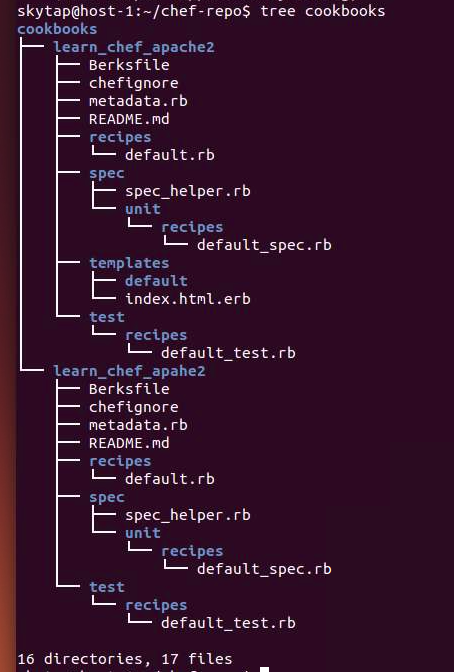
\includegraphics[width = 1.0\textwidth]{29.png}
\end{figure}
\begin{figure}[H]
  \centering
  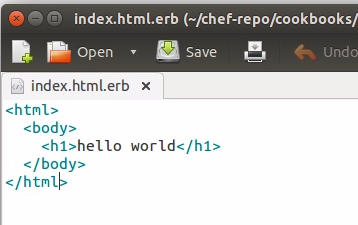
\includegraphics[width = 1.0\textwidth]{30.png}
\end{figure}
\begin{figure}[H]
  \centering
  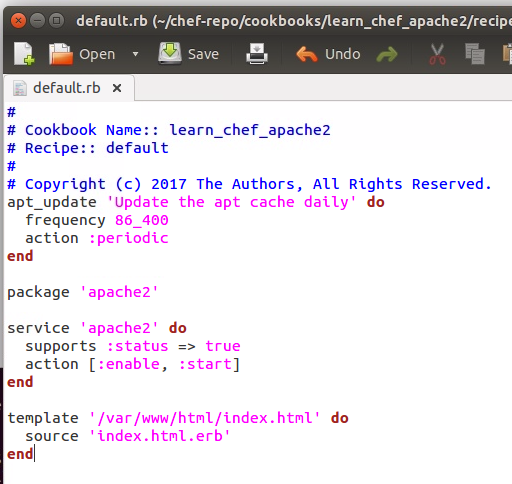
\includegraphics[width = 1.0\textwidth]{31.png}
\end{figure}
\begin{figure}[H]
  \centering
  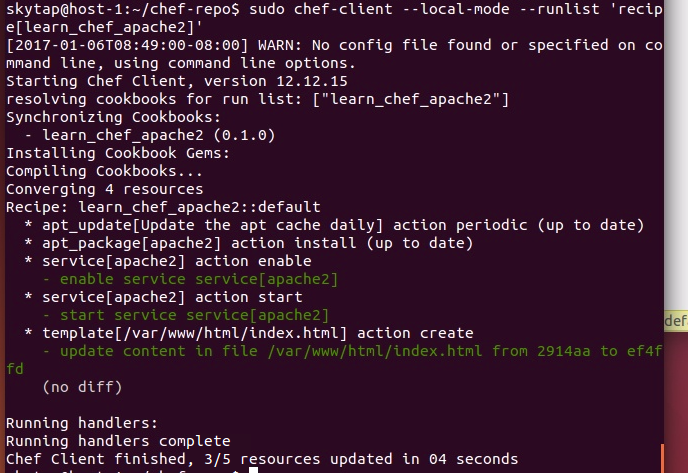
\includegraphics[width = 1.0\textwidth]{32.png}
\end{figure}
\begin{figure}[H]
  \centering
  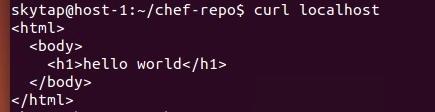
\includegraphics[width = 1.0\textwidth]{33.png}
\end{figure}
\begin{problem}[6. Explain in a few lines how chef enables the Infrastructure as Code paradigm]
\end{problem}
\newline
Programmers can just write a few lines of chef recipes code to set up the environment and configuration. Those recipe codes can run in different clients, which save the trouble of copying the whole VM file.
\newline
\begin{problem}[7. Image you are Rose-Hulman IT guy who figure all the vm for the students, will chef be fit in the situation?]
\end{problem}
\newline
Chef will be perfect for the Rose-Hulman student body since every Rose student have a similar VM/computer set up. Those set up can include Rose network configuration, SVN, Maple license etc. Instead of copying and paste the whole VM or computer file over, which costs a lot of time and space. Writing a chef recipes code which configures all the set up and just run those code in each VM or laptop will be super efficient. Chef also does version control so if there is update or new configuration, then just update the Chef receipe script then run again on the vm/laptop.
\end{document}